% Slides for 2024-07-30
% To create a slide, use the following:
% \begin{frame}{TITLE}
%     BODY
% \end{frame}

% To create a slide with a bullet list, use the following:
% \begin{frame}{TITLE}
%     \begin{itemize}
%         \item ITEM 1
%         \item ITEM 2
%     \end{itemize}    
% \end{frame}

% To create a slide with numbered list, use the following:
% \begin{frame}{TITLE}
%     \begin{enumerate}
%         \item ITEM 1
%         \item ITEM 2
%     \end{enumerate}
% \end{frame}

% To create a slide with a graphic:
% 1. Add the graphic to this folder (named picture.png)
% 2. Use the following:
% \begin{frame}{TITLE}
%     \centering
%     \includegraphics[height=0.7\textheight,width=0.7\textwidth,keepaspectratio]{picture.png}
% \end{frame}

% To create a slide with two columns, use the following:
% \begin{frame}{TITLE}
%     \begin{columns}
%         \begin{column}{0.5\textwidth}
%             COLUMN 1 BODY
%         \end{column}
%         \begin{column}{0.5\textwidth}
%             COLUMN 2 BODY
%         \end{column}
%     \end{columns}
% \end{frame}

\begin{frame}{Leaf: A Learnable Frontend}
    \centering
    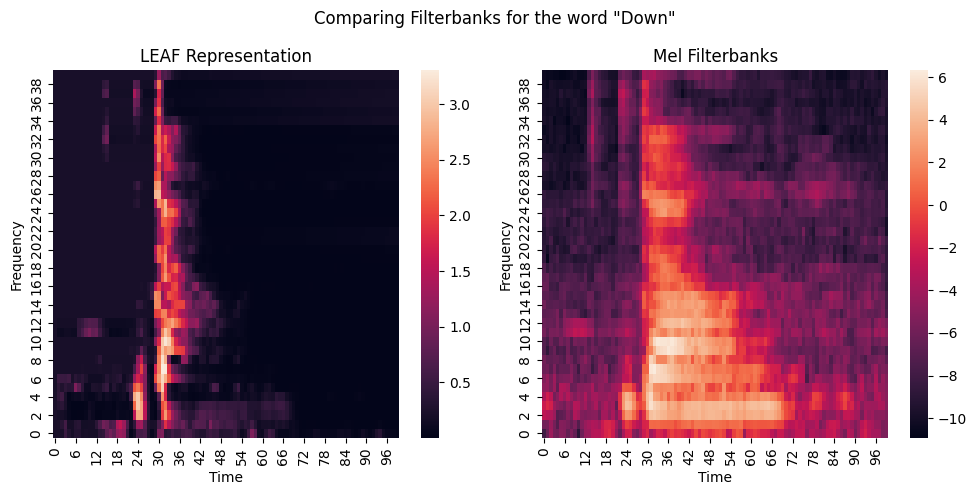
\includegraphics[height=0.7\textheight,width=0.9\textwidth,keepaspectratio]{images/leaf_demo.png}
\end{frame}
    
\begin{frame}{Leaf: A Learnable Frontend}
    \centering
    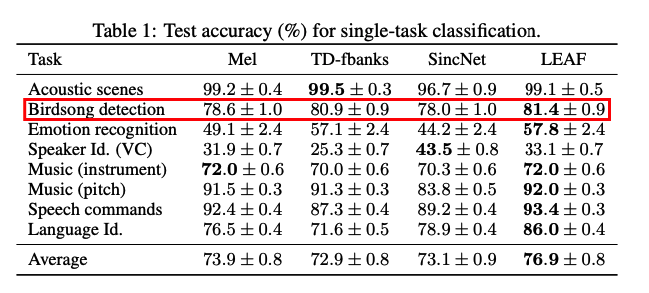
\includegraphics[height=0.7\textheight,width=0.9\textwidth,keepaspectratio]{images/leaf_results_paper.png}
\end{frame}

\begin{frame}{Complications}
    \begin{itemize}
        \item tf.keras.utils.audio\_dataset\_from\_directory()
        \item Tensorflow Datasets
        \item Some files causing ffmpeg errors
    \end{itemize}
\end{frame}

\begin{frame}{Current progress}
    \begin{itemize}
        \item Generated dataset using XC data
        \item Training their model to test viability
    \end{itemize}
\end{frame}

% jonathan

\begin{frame}{Audio Spectrogram Transformer}
    \centering
    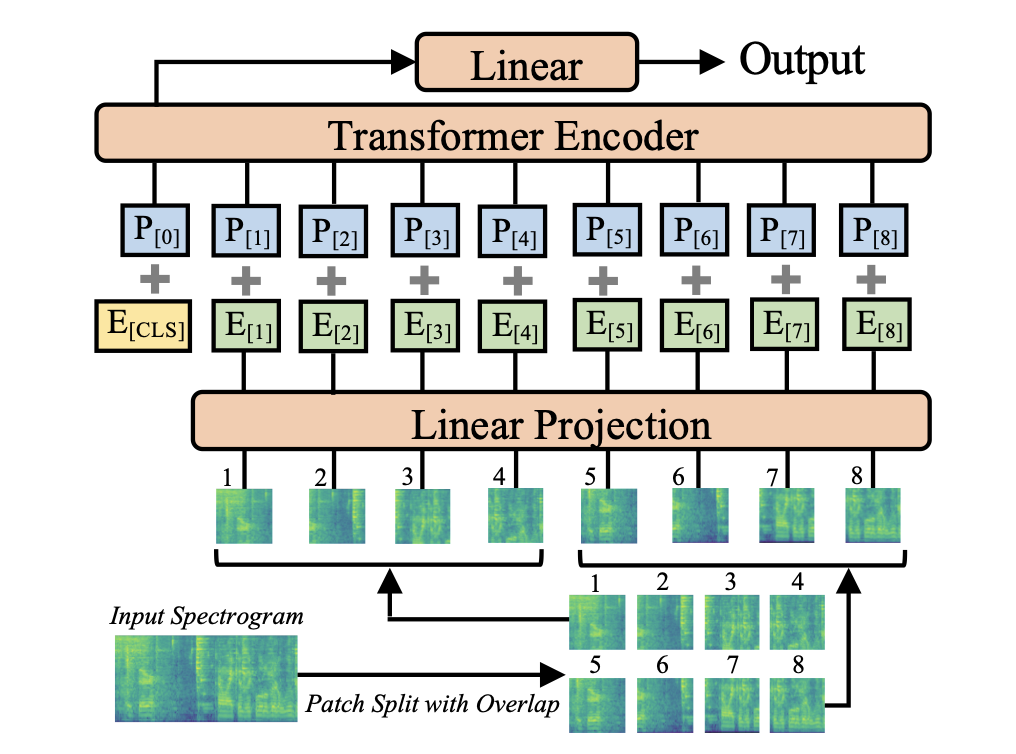
\includegraphics[height=0.7\textheight,width=0.9\textwidth,keepaspectratio]{images/ast.png}
\end{frame}

\begin{frame}{Progress}
    \centering
    \begin{columns}
            \begin{column}{0.5\textwidth}
                \begin{itemize}
                    \item Our Model: Timm Models
                    \item Our Dataset: PyTorch
                \end{itemize}
            \end{column}
            \begin{column}{0.5\textwidth}
                \begin{itemize}
                    \item AST: Custom training pipeline (script provided)
                    \item Script dataset: HuggingFace
                \end{itemize}
            \end{column}
    \end{columns}
\end{frame}

\begin{frame}{Conversion:}
    \centering
    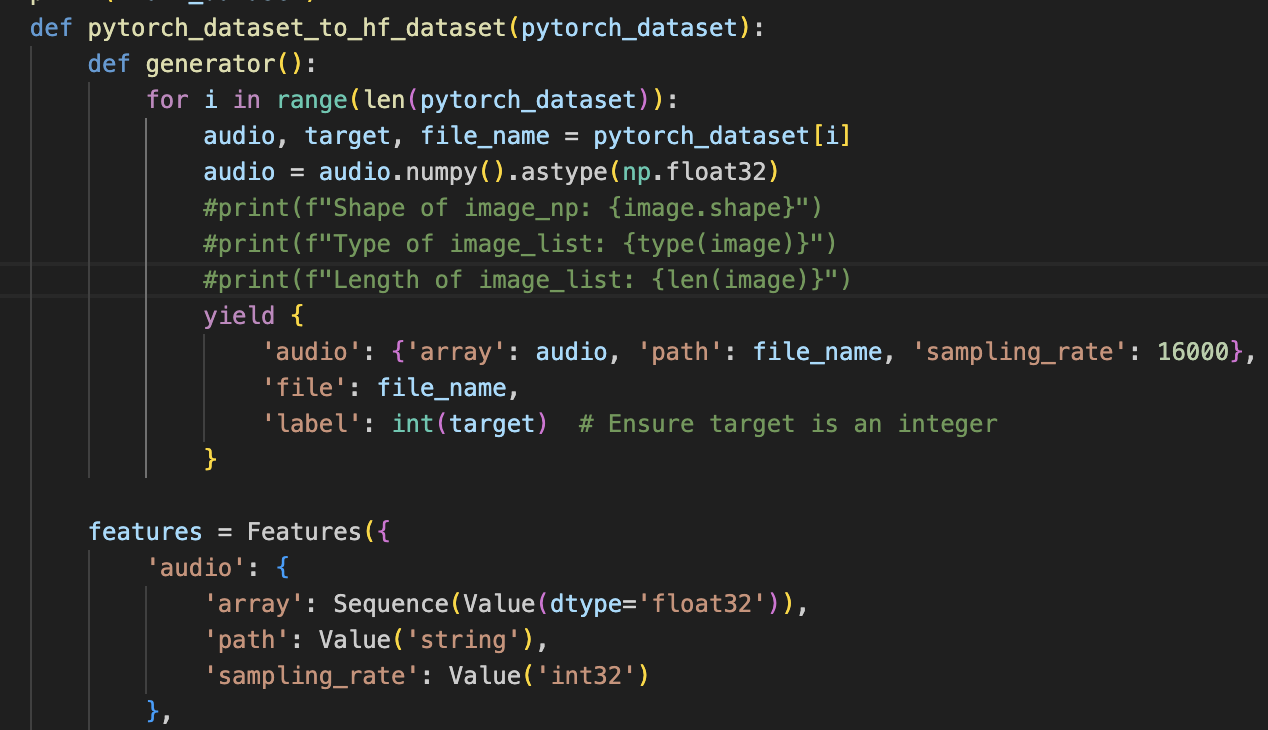
\includegraphics[height=0.7\textheight,width=0.9\textwidth,keepaspectratio]{images/converter.png}
    \begin{itemize}
        \item Problem: a lot of bugs :(
        \item label assignment
        \item extract audio from pipeline instead of spectrogram
    \end{itemize}
\end{frame}

%surangana

\begin{frame}{Created a Framework for the Home Page}
    \centering
    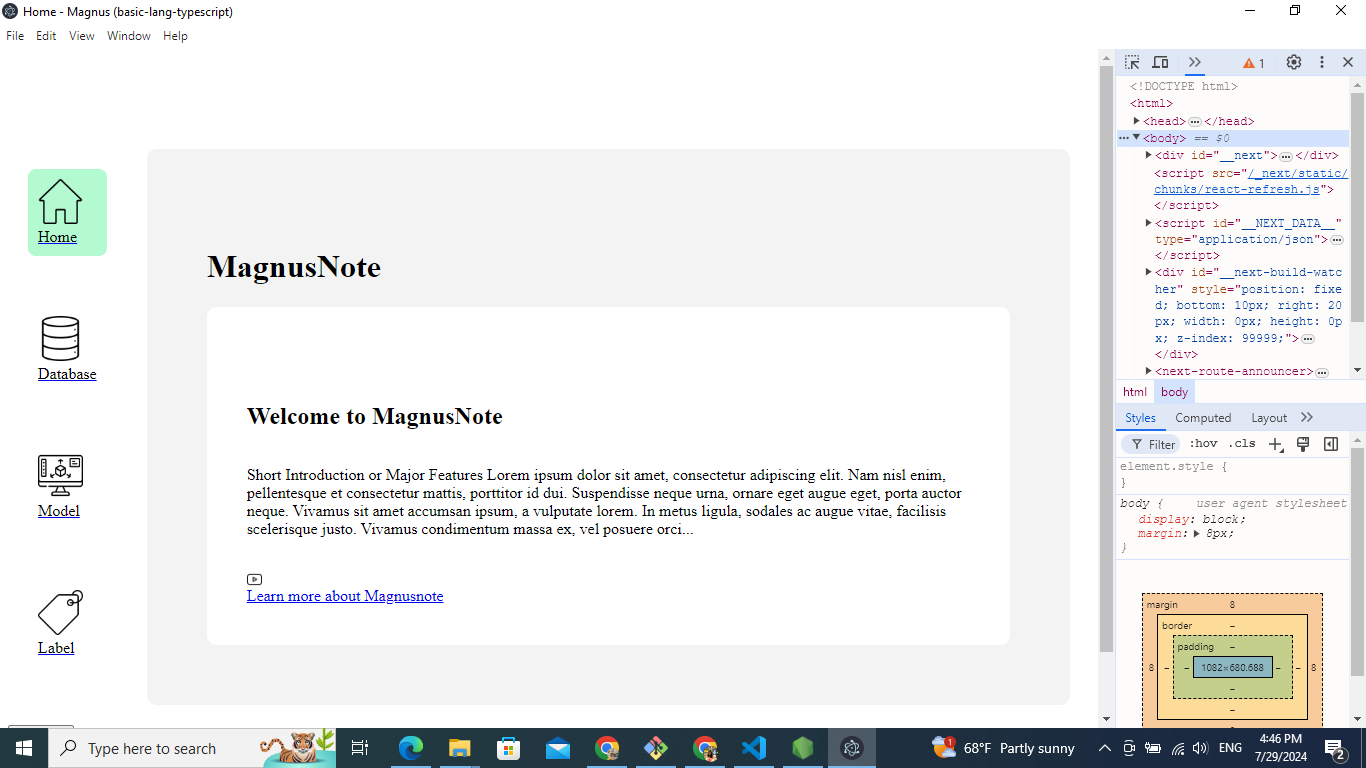
\includegraphics[height=0.7\textheight,width=0.7\textwidth,keepaspectratio]{homepage.png}  
\end{frame}

\begin{frame}{Created a Framework for the Database Page}
       \centering
       \begin{minipage}{0.45\textwidth}
            \centering
            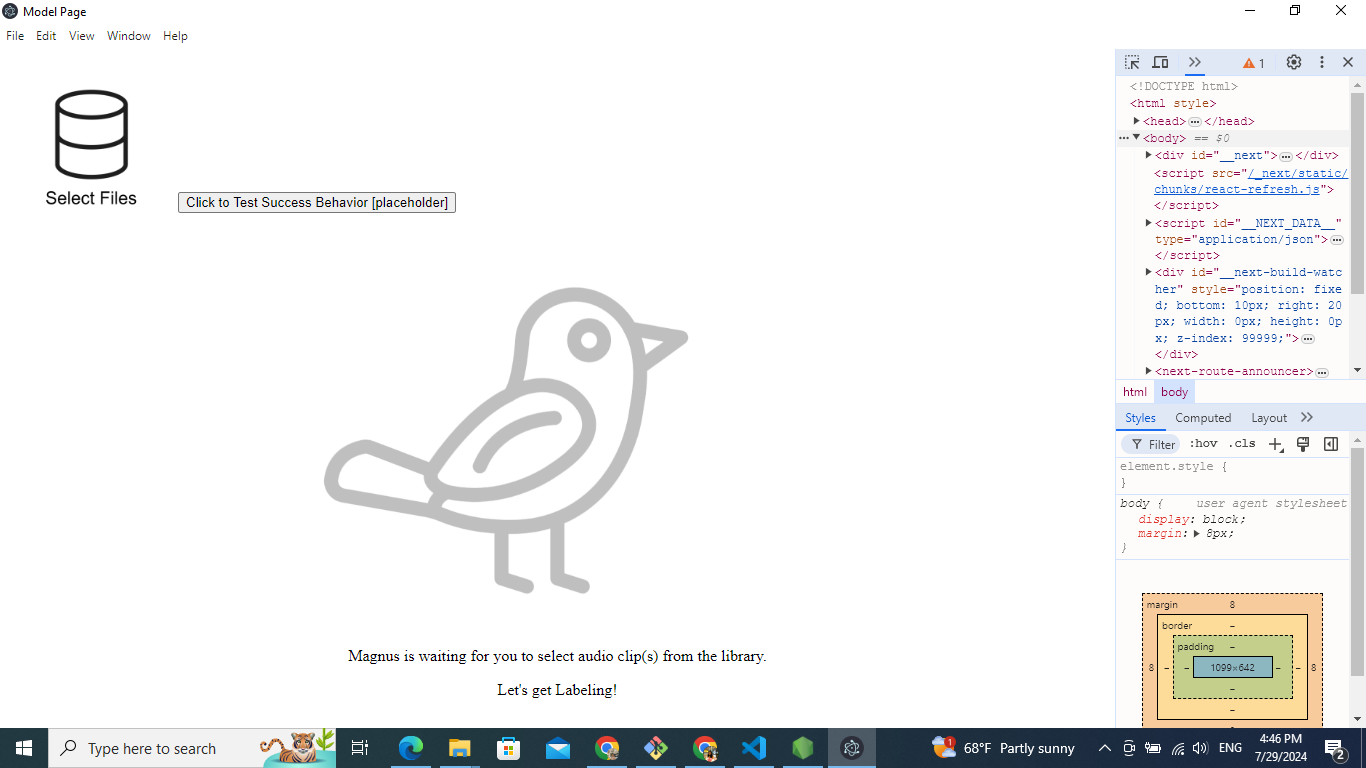
\includegraphics[width=\linewidth]{database1.png}
        \end{minipage}
        \hfill
        \begin{minipage}{0.45\textwidth}
            \centering
            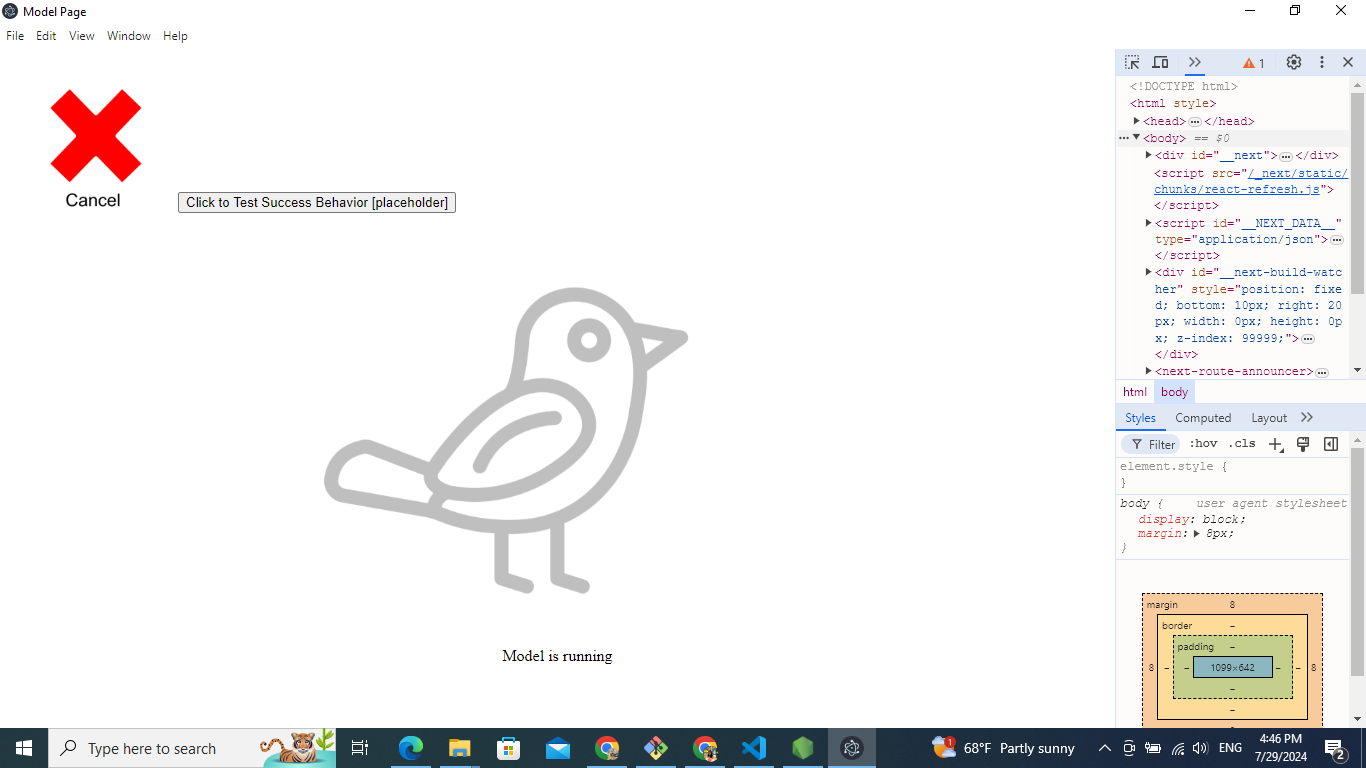
\includegraphics[width=\linewidth]{database2.png}
        \end{minipage}  
\end{frame}

\begin{frame}{Created a Framework for the Database Page}
    \centering
    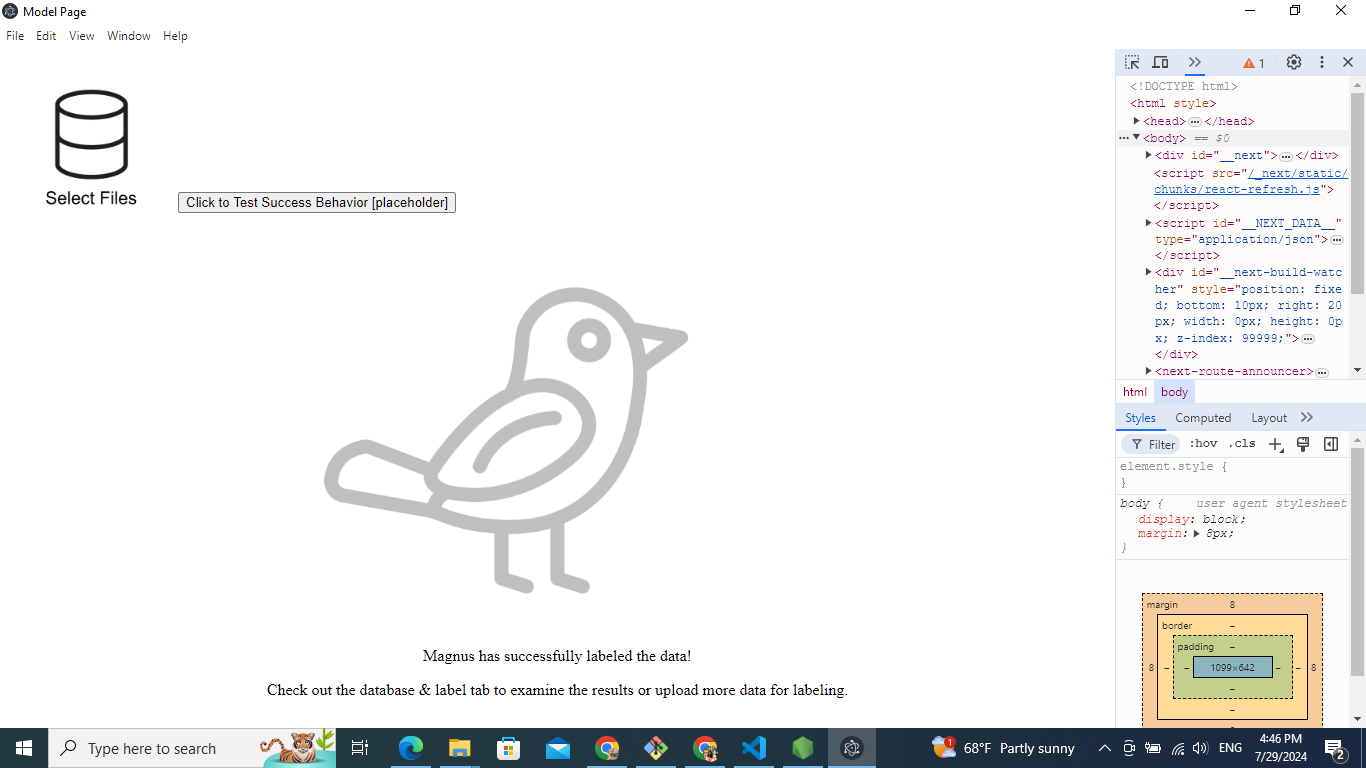
\includegraphics[height=0.7\textheight,width=0.7\textwidth,keepaspectratio]{database3.png}  
\end{frame}

\begin{frame}{Work in Progress}
    \begin{enumerate}
       \item Complete the Database Page
       \item Start working on the Labeling Page
   \end{enumerate}
\end{frame}
